\chapter{Observer模式}
\section{Observer模式的概念}
\subsection{定义}
观察者(Observer)模式的定义:指多个对象间存在一对多的依赖关系,当一个对象的状态发生改变时,所有依赖于它的对象都得到通知并被自动更新。这种模式有时又称作发布-订阅模式、模型-视图模式,它是对象行为型模式。
\subsection{优点}
\begin{enumerate}
	\item 降低了目标与观察者之间的耦合关系,两者之间是抽象耦合关系;
	\item 目标与观察者之间建立了一套触发机制。
\end{enumerate}
\subsection{缺点}
\begin{enumerate}
	\item 目标与观察者之间的依赖关系并没有完全解除,而且有可能出现循环引用。
	\item 当观察者对象很多时,通知的发布会花费很多时间,影响程序的效率。
\end{enumerate}
\subsection{观察者模式的角色}
\begin{enumerate}
	\item Subject观察对象:它提供了一个用于保存观察者对象的聚集类和增加、删除观察者对象的方法,以及通知所有观察者的抽象方法。
	\item ConcreteSubject具体观察对象:也叫具体目标类,它实现抽象目标中的通知方法,当具体主题的内部状态发生改变时,通知所有注册过的观察者对象。
	\item Observer观察者:它是一个抽象类或接口,它包含了一个更新自己的抽象方法,当接到具体主题的更改通知时被调用。
	\item ConcreteObserver具体观察者:实现抽象观察者中定义的抽象方法,以便在得到目标的更改通知时更新自身的状态。
\end{enumerate}
\subsection{应用场景}
\begin{enumerate}
	\item 对象间存在一对多关系,一个对象的状态发生改变会影响其他对象。
	\item 当一个抽象模型有两个方面,其中一个方面依赖于另一方面时,可将这二者封装在独立的对象中以使它们可以各自独立地改变和复用。
\end{enumerate}
\section{观察者模式实现——例一}
\begin{table}[!h]
	\begin{tabular}{|l|l|}
		\hline
		名字&说明\\
		\hline
		Observer&表示观察者接口\\
		\hline
		NumberGenerator&生成数值的对象的抽象类\\
		\hline
		RandomNumberGenerator&生成随机数的类\\
		\hline
		DigitObserver&以数字形式显示数值的类\\
		\hline
		GraphObserver&以简单的图示形式显示数值的类\\
		\hline
		Main&测试类\\
		\hline
	\end{tabular}
\end{table}
\begin{figure}[!h]
	\centering
	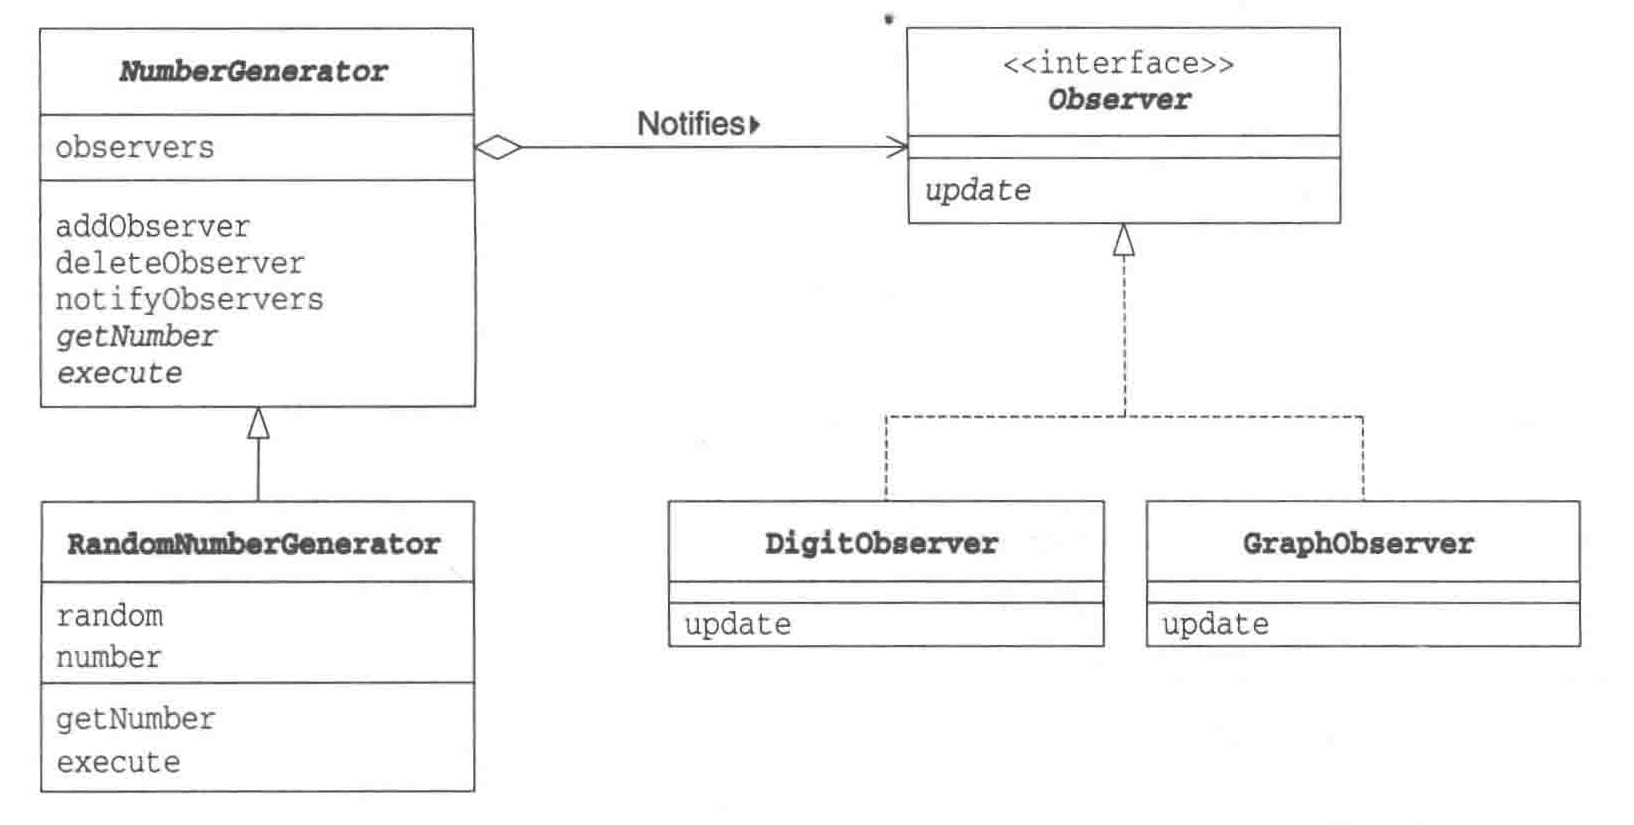
\includegraphics[width=0.8\textwidth]{image/17-1}
	\caption{观察者模式类图}
\end{figure}
\begin{lstlisting}
public interface Observer {
	//让被观察者通知观察者状态已经改变
	void update(NumberGenerator generator);
}
\end{lstlisting}
\begin{lstlisting}
//作为 Subject 被观察者
public abstract class NumberGenerator {
	private List<Observer> observers = new ArrayList<>();
	public void addObservers(Observer observer) {
		observers.add(observer);
	}
	public void deleteObserver(Observer observer) {
		observers.remove(observer);
	}
	// 向 Observer 发生通知
	public void notifyObserers() {
		Iterator<Observer> it = observers.iterator();
		while (it.hasNext()) {
			Observer o = it.next();
			o.update(this);
		}
	}
	//获取数值
	public abstract int getNumber();
	//生成数值
	public abstract void execute();
}
\end{lstlisting}
\begin{lstlisting}
// 以数字形式显示观察到的数值
public class DigitObserver implements Observer {
	public void update(NumberGenerator generator) {
		System.out.println("DigitObserver: " + generator.getNumber());
		try {
			Thread.sleep(100);
		} catch (InterruptedException e) {}
	}
}
// 将观察到的数值以 ***** 的方式显示出来
public class GraphObserver implements Observer {	
	public void update(NumberGenerator generator) {
		System.out.print("GraphObserver: ");
		int count = generator.getNumber();
		for (int i = 0; i < count; i++) {
			System.out.print("*");
		}
		System.out.println();
		try {
			Thread.sleep(100);
		} catch (InterruptedException e) {}
	}
}
\end{lstlisting}
\begin{lstlisting}
public class RandomNumberGenerator extends NumberGenerator {
	private Random random = new Random();
	private int number;
	public int getNumber() {
		return number;
	}
	public void execute() {
		for (int i = 0; i < 20; i++) {
			number = random.nextInt(50);
			notifyObserers();
		}
	}
}
\end{lstlisting}
\begin{lstlisting}
public class Main {
	public static void main(String[] args) {
		NumberGenerator generator = new RandomNumberGenerator();
		Observer observer1 = new DigitObserver();
		Observer observer2 = new GraphObserver();
		generator.addObservers(observer1);
		generator.addObservers(observer2);
		generator.execute();
	}
}
\end{lstlisting}
\section{观察者模式实现——例二}
\begin{figure}[!h]
	\centering
	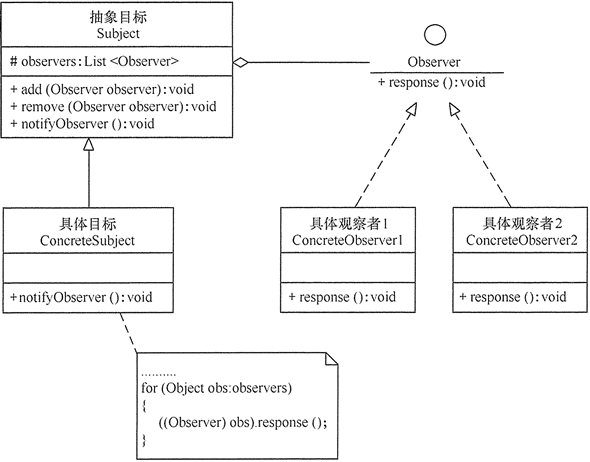
\includegraphics[width=0.8\textwidth]{image/17-2}
	\caption{观察者模式的结构图}
\end{figure}
\begin{lstlisting}
//抽象观察者
interface Observer {
	void response(); //反应
}

//具体观察者1
class ConcreteObserver1 implements Observer {
	public void response() {
		System.out.println("具体观察者1作出反应!");
	}
}

//具体观察者2
class ConcreteObserver2 implements Observer {
	public void response() {
		System.out.println("具体观察者2作出反应!");
	}
}
\end{lstlisting}
\begin{lstlisting}
//抽象目标
abstract class Subject {
	protected List<Observer> observers = new ArrayList<Observer>();
	//增加观察者方法
	public void add(Observer observer) {
		observers.add(observer);
	}
	//删除观察者方法
	public void remove(Observer observer) {
		observers.remove(observer);
	}
	public abstract void notifyObserver(); //通知观察者方法
}

//具体目标
class ConcreteSubject extends Subject {
	public void notifyObserver() {
		System.out.println("具体目标发生改变...");
		System.out.println("--------------");
		for (Object obs : observers) {
			((Observer) obs).response();
		}
	}
}
\end{lstlisting}
\begin{lstlisting}
public class ObserverPattern {
	public static void main(String[] args) {
		Subject subject = new ConcreteSubject();
		Observer obs1 = new ConcreteObserver1();
		Observer obs2 = new ConcreteObserver2();
		subject.add(obs1);
		subject.add(obs2);
		subject.notifyObserver();
	}
}
\end{lstlisting}
\begin{lstlisting}
//output
具体目标发生改变...
--------------
具体观察者1作出反应!
具体观察者2作出反应!
\end{lstlisting}

\section{模式扩展——java.util.Observer}
\subsection{Observable类}
Observable 类是抽象目标类,它有一个 Vector 向量,用于保存所有要通知的观察者对象。
\begin{itemize}
	\item void addObserver(Observer o) 方法:用于将新的观察者对象添加到向量中。
	\item void notifyObservers(Object arg) 方法:调用向量中的所有观察者对象的 update。方法,通知它们数据发生改变。通常越晚加入向量的观察者越先得到通知。
	\item void setChange() 方法:用来设置一个 boolean 类型的内部标志位,注明目标对象发生了变化。当它为真时,notifyObservers() 才会通知观察者。
\end{itemize}
\subsection{Observer接口}
Observer 接口是抽象观察者,它监视目标对象的变化,当目标对象发生变化时,观察者得到通知,并调用 void update(Observable o,Object arg) 方法,进行相应的工作。
\subsection{实现原油期货例子}
\begin{figure}[!h]
	\centering
	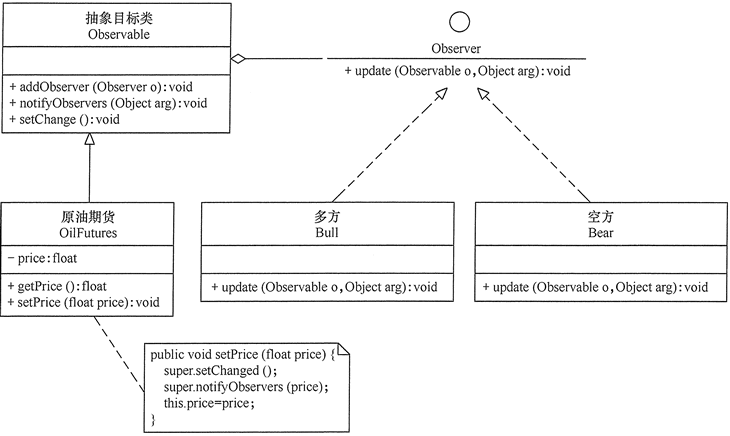
\includegraphics[width=0.8\textwidth]{image/17-3}
	\caption{实现类图}
\end{figure}
\begin{lstlisting}
//具体目标类:原油期货
class OilFutures extends Observable {
	private float price;
	public float getPrice() {
		return this.price;
	}
	public void setPrice(float price) {
		super.setChanged();  //设置内部标志位,注明数据发生变化 
		super.notifyObservers(price);    //通知观察者价格改变了 
		this.price = price;
	}
}
\end{lstlisting}
\begin{lstlisting}
//具体观察者类:多方
class Bull implements Observer {
	public void update(Observable o, Object arg) {
		Float price = ((Float) arg).floatValue();
		if (price > 0) {
			System.out.println("油价上涨" + price + "元,多方高兴了!");
		} else {
			System.out.println("油价下跌" + (-price) + "元,多方伤心了!");
		}
	}
}

//具体观察者类:空方
class Bear implements Observer {
	public void update(Observable o, Object arg) {
		Float price = ((Float) arg).floatValue();
		if (price > 0) {
			System.out.println("油价上涨" + price + "元,空方伤心了!");
		} else {
			System.out.println("油价下跌" + (-price) + "元,空方高兴了!");
		}
	}
}
\end{lstlisting}
\begin{lstlisting}
public class CrudeOilFutures {
	public static void main(String[] args) {
		OilFutures oil = new OilFutures();
		Observer bull = new Bull(); //多方
		Observer bear = new Bear(); //空方
		oil.addObserver(bull);
		oil.addObserver(bear);
		oil.setPrice(10);
		oil.setPrice(-8);
	}
}
\end{lstlisting}
\begin{lstlisting}
//output
油价上涨10.0元,空方伤心了!
油价上涨10.0元,多方高兴了!
油价下跌8.0元,空方高兴了!
油价下跌8.0元,多方伤心了!
\end{lstlisting}
\section{思路扩展}
\begin{enumerate}
	\item 可替换性(复用)实现:
	\begin{itemize}
		\item 利用抽象类和接口从具体类中抽出抽象方法;
		\item 将实例作为参数传递至类中,或者在类中的字段保存实例,不适用具体类型,而是使用抽象类型和接口。
	\end{itemize}
	\item Observer顺序例一中先注册先调用,但java的Observer相反。
	\item 避免循环调用。
	\item 传递信息的方式:
	\begin{itemize}
		\item 仅传递Subject,可以通过Subject获取数据;
		\item 数据、Subject都传递,会降低灵活性;
		\item 传递数据,一对多不适用。
	\end{itemize}
	\item 发布——订阅更适合。
	\item MVC中一个Model对应多个View也是类似观察者模式。
\end{enumerate}
\section{相关设计模式}
\noindent\textbf{Mediator模式}
\begin{itemize}
	\item 在Mediator中,有时使用Observer来实现Mediator角色和Colleague角色之间通信;
	\item Mediator虽然会发送通知,但是为了对Colleague角色进行仲裁;
	\item Observer将Subject角色的状态变化通知给Observer角色目的是为了使得二者同步。
\end{itemize}